
%%%%%%%%%%%%%%%%%%%%%%%%%%%%%%%%%%%%%%%%%%%%%%%%%%%%%%%%%%%%%%%%%%%%%%%%%%%%
% This will help you in writing your homebook
% Remember that the character % is a comment in latex

% Divide the work you have done in each of the chapters used
% during the lab lessons in a new chapter, as in the example below,
% using a coherent title


% For each chapter you can include :

%-----------------------------
% VHDL file, using the sintax:


	%\begin{listato}
	%\lstinputlisting{./exeMPLE/listato1.vhd}
	%\end{listato}

% the path to the file must be correct, obviously
% Should you have listings written in other languages the method is the
% same, but the language set up must be changed using a different
% setting for the command \lstset{language=VHDL} in file homebook.tex


%-----------------------------
% figures in postcript (ps) or encapsulated postcript (eps)
% format, using the syntax:

%	\begin{figure}[h]
%	\centering
%	\includegraphics[width=9cm]{./cap1/figure1.eps}
%	\caption{Put a caption if you want (didascalia...:)))}
%	\label{put-a-label-for-referring-to-this-picture}
%	\end{figure}

% the path to the file must be correct, obviously
% you can refer to this picture in any point of your document
% by typing the instruction:

% 	\ref{put-a-label-for-referring-to-this-picture}

% that is using the same label you put in the fiure label
% when you will run the "latex command" an automatic reference to
% this figure with the correct enumeration will be inserted


%-----------------------
% comment in text format (if you are not skilled in latex and don't want to be)
% using the sintax:

	%\begin{verbatim}
	% blablabla
	%\end{verbatim}

% The verbatimg includes text as it is, as you could write in a normal text file

% (BETTER) If uou want to write enhancing all the latex possibilities you
% should add to you text a few commands in some particular cases.
% In the following you have and example of a few chapters roughtly commented
% and written all in this file: remember that you can saparate
% each chapter in different files (this is always what a latex pro does)
% and include them using the instruction: \input{./directoryxx/fileyy.tex}


%%%%%%%%%%%%%%%%%%%%%%%%%%%%%%%%%%%%%%%%%%%%%%%%%%%%%%%%%%%%%%%%%%%%%%%%%%%%%%%
%%%%%%%%%%%%%%%%%%%%%%%%%%%%%%%%%%%%%%%%%%%%%%%%%%%%%%%%%%%%%%%%%%%%%%%%%%%%%%%%%
%%%%%%%%%%%%%%%%%%%%%%%%%%%%%%
% Beginning of latex commands
% You can copy this in a new file (e.g. cap1/cap1.tex) and inlcude it here
% using the command : \input{./cap1/cap1.tex}



\chapter{Lab 1: design and implementation of a digital filter}
{\let\thefootnote\relax\footnote{{\href{https://github.com/campandrea/Lab_ISA/}{\textcolor{black}{Github repository:} https://github.com/campandrea/Lab\_ISA/}}}}
\section{Reference model development}
\subsection{Design of a digital IIR filter direct form II}

\subsubsection{Filter design and coefficients quantization using Matlab}
The delivery of the laboratory required the development of an IIR digital filter with direct form II architecture with the following features:
\begin{itemize}
\item Frequenza di taglio $F_{T} = 2 kHz$
\item Numero di bit $N_{b} = 10$
\item Ordine del filtro $N = 1$
\item Total Harmonic Distorsion $THD \leq -30 dB$
\end{itemize}

Osservando l'equazione che descrive il comportamento del filtro IIR:
\begin{equation}
y(n) = \sum_{i=0}^N a_{i}x[n-i]  + \sum_{j=1}^N b_{j}y[n-j]
\end{equation}

si può evincere la dipendenza dell'uscita del filtro in funzione dei coefficienti $a_{i}$ e $b_{j}$, questi sono necessari e definiscono il comportamento globale del filtro IIR, pertanto è stato necessario utilizzare dei tools per la loro computazione. A tal fine si è ricorso a Matlab, usando gli scripts resi disponibili sul \textit{Portale della didattica}: \textit{my\_iir\_filter.m} e \textit{myiir\_design.m}. Tali files hanno fatto uso della funzione \textit{butter}, che genera i coefficienti del filtro digitale con risposta Butterworth(massimamente piatta), noti l'ordine del filtro desiderato e la frequenza di taglio normalizzata rispetto alla frequenza di Nyquist. I coefficienti quantizzati a $10 bits$ ottenuti sono i seguenti:

\begin{itemize}
\item $a = $[512 -82]
\item $b = $[215 215]
\end{itemize}

Lo script di Matlab ha generato inoltre un'implementazione del filtro per mostrare la risposta a due segnali in ingresso, uno dentro la banda e l'altro fuori dalla banda; inoltre ha prodotto il grafico della risposta in frequenza del filtro:
\begin{figure}[H]
\centering
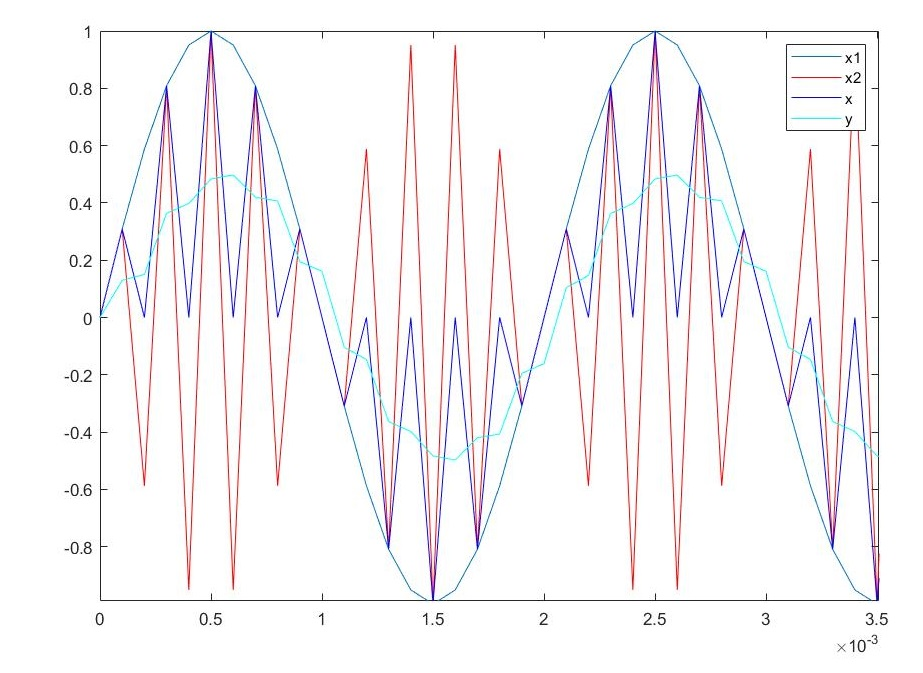
\includegraphics[width= 11cm]{IIR_IO.jpg}
\caption{Segnali di Input e Output del Filtro}
\label{fig:IO_signals}

\end{figure}
I segnali $x_{1}$ e $x_{2}$ sono rispettivamente il segnale dentro la banda e il segnale fuori dalla banda, il segnale $x$ è invece la media tra i due ed è quest'ultimo ad essere stato dato in ingresso al filtro nello script di Matlab. Come si vede infatti dall'uscita, il filtro si è comportato esattamente come un passa-basso, lasciando passare solo la componente in bassa frequenza shiftata e attenuata.
In seguito invece, è rappresentata la risposta Butterworth in funzione della frequenza normalizzata, del filtro IIR digitale
\begin{figure}[H]
\centering
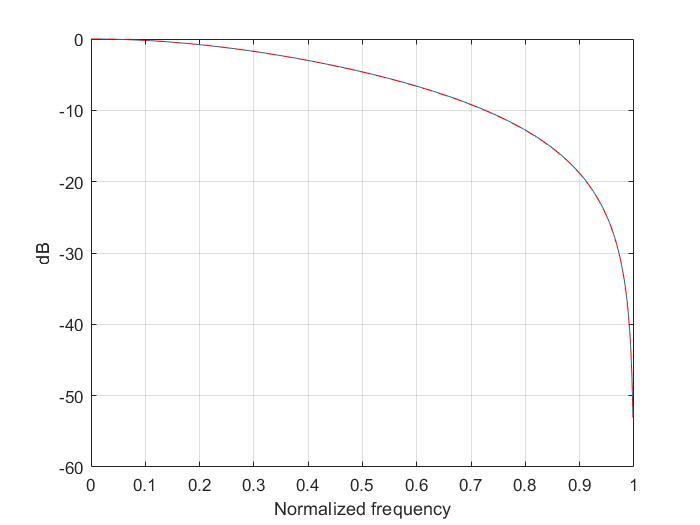
\includegraphics[width= 11cm]{IIR_responce.jpg}
\caption{Risposta Butterworth del filtro IIR}
\label{fig:Butterworth}
\end{figure}

\subsubsection{Fixed point C models}

In seguito allo sviluppo del filtro IIR in ambiente Matlab, è stata implementata una versione in linguaggio C per valutare le prestazioni del filtro in aritmetica \textit{Fixed-point}. A tale scopo è stato utilizzato il programma in linguaggio C disponibile sul \textit{Portale della didattica} chiamato \textit{myfilterii.c}, al quale sono stati passati da linea di comando il file dei campioni generati da Matlab e il file su cui salvare i campioni in uscita dal filtro implementato in linguaggio C. Il programma ha prodotto un file di uscita che è stato poi analizzato in ambiente Matlab per valutarne il Total Harmonic Distorsion(THD). Avendo scelto una rappresentazione iniziale dei coefficienti a 10 bits, sono stati ricavati i seguenti THDs rispettivamente con il segnale di uscita ricavato su Matlab e in seguito ricavato in aritmetica Fixed point in C:

\begin{figure}[H]
\centering
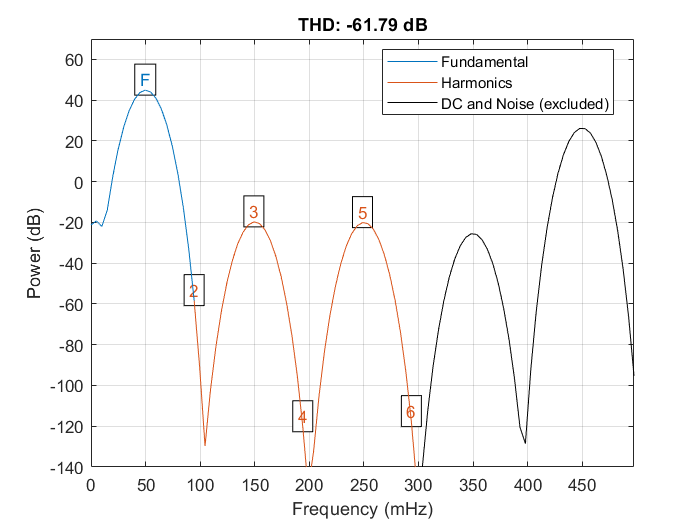
\includegraphics[width= 11cm]{THD_10_bit_matlab_result.png}
\caption{THD con aritmetica Floating point}
\label{fig:THD_10_bit_FL_P}
\end{figure}

\begin{figure}[H]
\centering
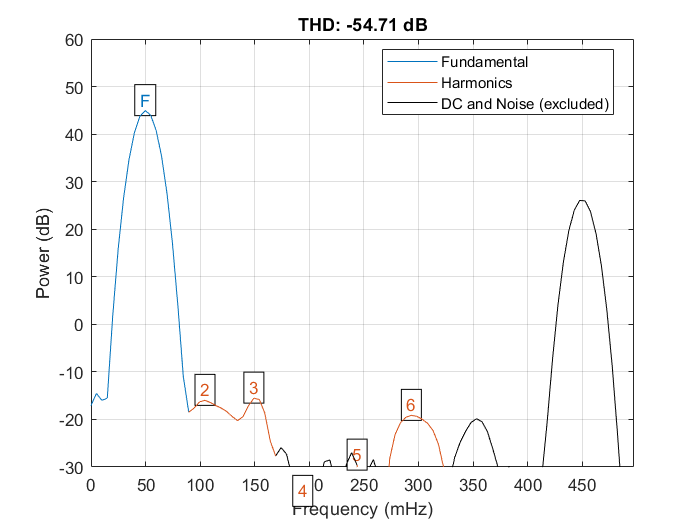
\includegraphics[width= 11cm]{THD_10_bit_C_result.png}
\caption{THD con aritmetica Fixed point a 10 Bits}
\label{fig:THD_10_bit_FIX_P}
\end{figure}

Come si può osservare dai grafici sopra, il Total Harmonic Distorsion del filtro che ha fatto uso di coefficienti e del segnale rappresentati su 10 bits è troppo elevato rispetto alle specifiche assegnate. Pertanto è stato iterato il processo descritto sopra, utilizzando ad ogni ciclo un bit in meno nella rappresentazione, sino a che non è stato ricavato il valore ottimale di bits che permettesse di rimanere all'interno delle specifiche del \textit{THD}, il quale corrisponde a 5 bits.
In seguito sono stati riportati i grafici dei THDs, rispettivamente calcolati con il segnale di uscita ricavato su Matlab e a seguire quello valutato con l'aritmetica Fixed point in C:

\begin{figure}[H]
\centering
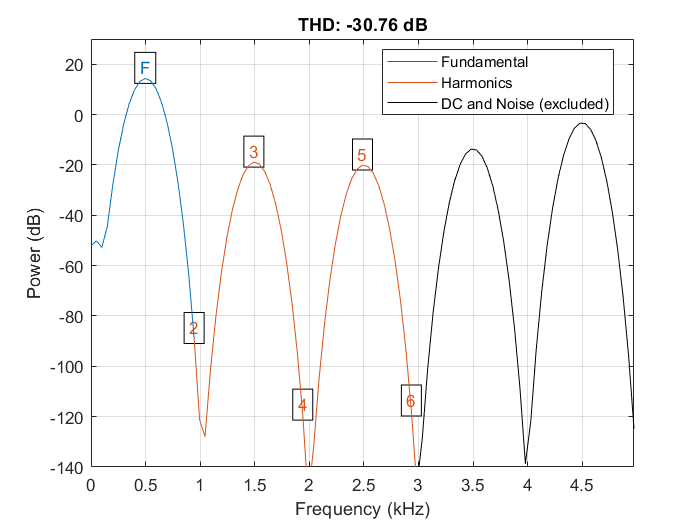
\includegraphics[width= 11cm]{THD_5_bit_matlab_result.png}
\caption{THD con aritmetica Floating point}
\label{fig:THD_5_bit_FIX_P}
\end{figure}

\begin{figure}[H]
\centering
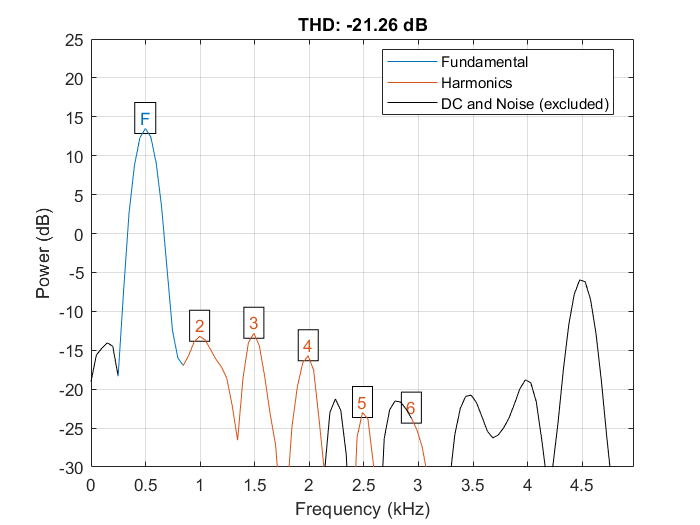
\includegraphics[width= 11cm]{THD_5_bit_C_result.png}
\caption{THD con aritmetica Fixed point a 5 Bits}
\label{fig:THD_5_bit_FIX_P}
\end{figure}

Il valore finale del THD è pertanto $-21.26 dB$ il quale è perfettamente consono alle specifiche di progetto assegnate.

\subsection{Advanced architecture development: J-look-ahead}

In questa sezione verrà discussa l'analisi preliminare relativa al progetto del filtro IIR, al quale è stata applicata la tecnica del look-ahead al fine di incrementare le prestazioni del sistema. Nelle sezioni successive verrà accuratamente discusso come questi miglioramenti sono stati implementati e verrà presentata una dimostrazione per raggiungere il risultato finale che viene anticipato al fine di presentare esclusivamente l'analisi del modello. In seguito si può osservare l'immagine del filtro IIR modificato:

\begin{figure}[H]
\centering
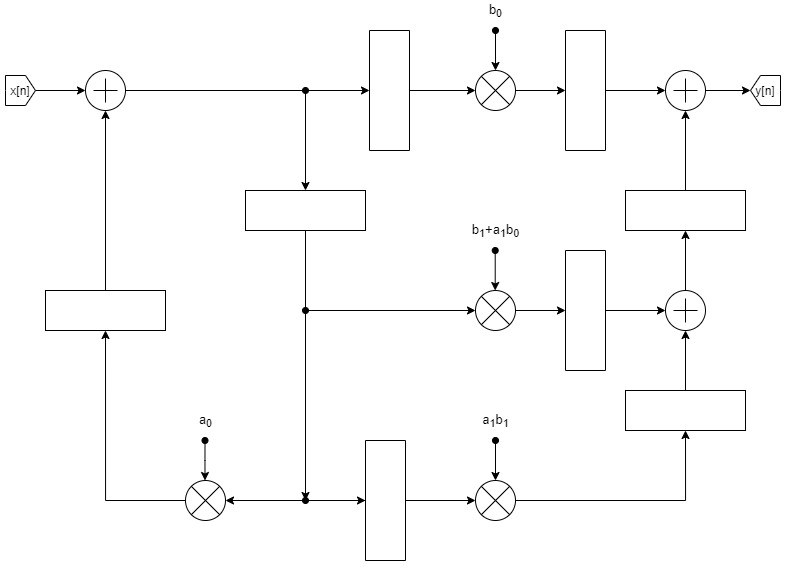
\includegraphics[width= 11cm]{J-look-ahead.png}
\caption{Architettura del Filtro IIR J-Look-Ahead}
\label{fig:IIR_JLA}
\end{figure}

Per il circuito di cui sopra, è stato creato un modello in C per l'analisi in Fixed point; per tale modello si è fatto ricorso ad un nuovo script scritto ad hoc, che utilizza un vettore di 7 componenti per simulare l'architettura pipelinata del componente. Il nome dello script è \textit{J-look-ahead.c} ed stato incluso nella consegna della relazione. Il segnale in uscita dal filtro è stato poi analizzato su Matlab per valutarne la bontà e per prima cosa è stato valutato il Total Harmonic Distorsion che, si può osservare dalla seguente immagine sia rimasto perfettamente all'interno delle specifiche:

\begin{figure}[H]
\centering
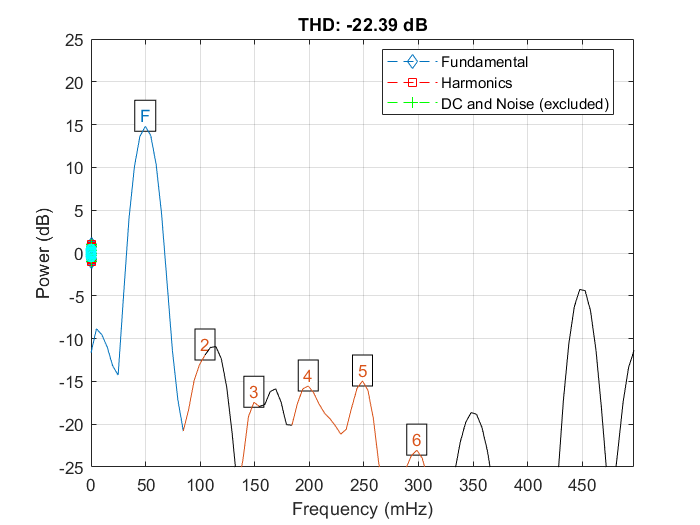
\includegraphics[width= 11cm]{JLAH_THD_5_bit_C_result.png}
\caption{THD del filtro IIR J-Look-Ahead}
\label{fig:THD_5_bit_IIR_JLA}
\end{figure}

\subsubsection{Comparing Direct form II and J-Look-Ahead}
Ciò che verrà presentata ora è un'analisi dei dati ottenuti dai due filtri, con lo scopo di dimostrarne l'equivalenza nel comportamento nonostante la grande differenza tra le due topologie. In particolare verranno esaminati in ambiente Matlab:

\begin{itemize}
\item Valori iniziali dei segnali
\item Media dei due segnali
\item Varianza dei due segnali
\end{itemize}

Per cominciare si nota che la topologia del filtro IIR look-ahead presenta due stadi di Pipe che si interpongono tra il segnale di ingresso e l'uscita, questo implica che il segnale ha sicuramente una latenza superiore rispetto alla topologia Direct form II, che corrisponde esattamente a due cicli del clock. La tabella sottostante conferma infatti la veridicità della precedente asserzione:



\begin{table}[H]
\begin{center}
\begin{tabular}{|c|c|}
\hline
Direct Form II	& J-Look-Ahead 			\\ \hline
$0$  			& $0$                 	\\ \hline
$1$      		& $0$                 	\\ \hline
$1$     		& $0$                 	\\ \hline
$4$      		& $1$                  	\\ \hline
$5$      		& $1$                  	\\ \hline
$7$      		& $5$                 	\\ \hline
$6$     		& $5$                   \\ \hline
$4$      		& $6$                   \\ \hline
$4$      		& $6$                   \\ \hline
\end{tabular}
\end{center}
\end{table}

Come il grafico del \textit{THD} del J-look-Ahead ha anticipato, i due segnali non sono perfettamente identici nei valori e nonostante l'andamento complessivo possa essere molto simile, ci si può interessare quanto esso sia effettivamente differente, perciò si rivela a questo punto necessaria un'analisi dei segnali in uscita dai due filtri di carattere qualitativo e quantitativo. In seguito sono rappresentati i valori di Media e Varianza dei due segnali:

\begin{table}[H]
\begin{center}
\begin{tabular}{|c|c|c|}
\hline
Parametro		& Direct Form II	& J-Look-Ahead 			\\ \hline
Media			&$-0.8308$  		& $-2.2537$	           	\\ \hline
Varianza		&$23.6312$      	& $32.9303$             \\ \hline

\end{tabular}
\end{center}
\end{table}

Come precedentemente detto, i due segnali non sono perfettamente uguali, e infatti presentano media e varianza altrettanto differenti che però presentano  stesso ordine di grandezza e valori coerenti con il sistema in analisi. Per un'analisi più fine è però necessario l'ausilio della varianza di Allan, per misurare quanto il rumore vada a degradare le prestazioni e quanto il comportamento oscillatorio dell'uscita sia più o meno stabile. In seguito sono rappresentate le varianze dei due segnali e la differenza tra le due varianze per valutare quanto la stabilità di Direct Form II differisce da quella del J-Look-Ahead, entrambi i grafici sono stati generati utilizzando la funzione Matlab \textit{allanvar()}:

\begin{figure}[H]
\centering
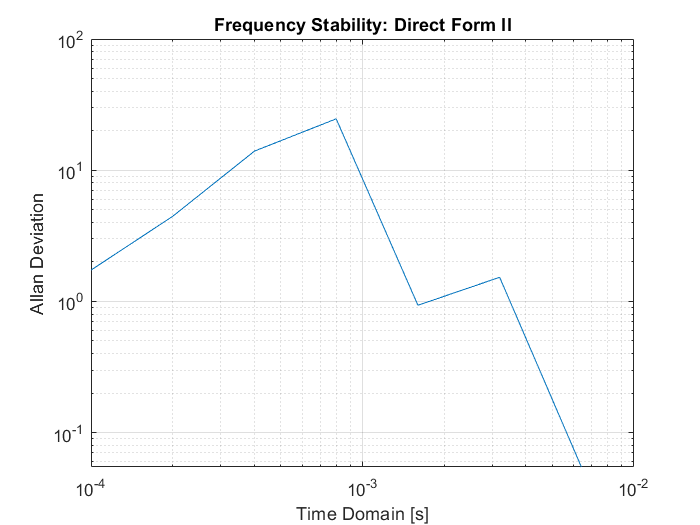
\includegraphics[width= 11cm]{Allan Var DF2.png}
\caption{Varianza di Allan del Filtro IIR Direct Form II}
\label{fig:Allan_Var_DF2}
\end{figure}

\begin{figure}[H]
\centering
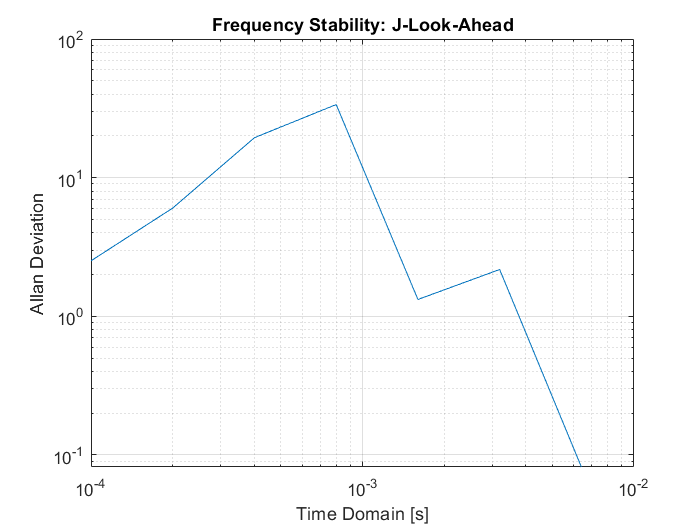
\includegraphics[width= 11cm]{Allan Var JLA.png}
\caption{Varianza di Allan del Filtro IIR J-Look-Ahead}
\label{fig:Allan_Var_JLA}
\end{figure}

\begin{figure}[H]
\centering
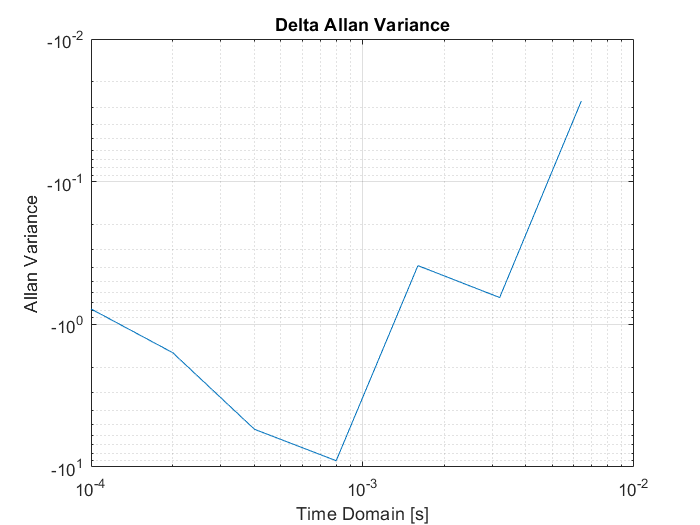
\includegraphics[width= 11cm]{Allan Var difference.png}
\caption{Differenza della Varianza di Allan}
\label{fig:Allan_Var_difference}
\end{figure}

Dai grafici in figura \autoref{fig:Allan_Var_DF2} e \autoref{fig:Allan_Var_JLA}, si può notare come nella prima metà della finestra di osservazione il segnale abbia un rumore elevato, generando una bassa stabilità dell'oscillatore, ma che con il passare del tempo sembra andare ad affievolirsi aumentandone appunto la stabilità in frequenza. Dalla differenza dei due grafici invece possiamo notare che il comportamento in frequenza dei due segnali è molto simile, in quanto la differenza delle loro varianze è molto al di sotto dell'ordine di grandezza dell'unità.

\section{Second Section}
\todo{insert the second section here}


\begin{table}[h]
\begin{center}
\begin{tabular}{|l|l|l|}
\hline
Architercture & period_min ns & area (um^2)\\
\hline
classic & 1.56 & 4047.7\\
\hline
csa & 4.28 & 4851.6\\
\hline
pparch & 1.45 & 4088.4\\
\hline
stage2 reg+compile & 0.79 & 4924.7\\
\hline
stage2 reg+compile\_ultra & 1.52 & 4188.2\\
\hline
mbe compile & 1.94 & 5360.4\\
\hline
mbe compile ultra & 1.64 & 5327.7\\
\hline
\end{tabular}
\end{center}
\caption{Questa e' la caption}
\label{tab:tab_label}
\end{table}




% include here only file for the third lesson and homeworks
% here the path to figures and VHDL should be ./exe3/
